\documentclass{school-22.211-notes}
\date{March 14, 2012}

\begin{document}
\maketitle

%%%%%%%%%%%%%%%%%%%%%%%%%%%% Exam 1 Review Begin %%%%%%%%%%%%%%%%%%%%%%%%%%%%%%%%%%%%%%%%%%
\lecture{Exam 1 Review}
Know how to interprete thermal scattering pdf and cdf. Questions would be based on understanding of the physics. 
\topic{Part 1: Background Info (see Ch 1-3 from Reuss)}
\begin{enumerate}
\item Number Density, flux, lethargy.  
\item Mean free path
\item 1/v absorption cross section: 
  \begin{itemize}
  \item Wave-particle duality suggests that slow neutrons see a larger portion of space than fast neutrons, which means that slow neutrons often have larger cross sections, which leads to the 1/v rule for absorption (Reuss, 2.4.1). 
  \item Reason: Breit-Wigner states that absorption cross section is ($i = \gamma$ for radiative capture and $f$ for fission etc):
    \eqn{ \sigma_i = \pi \bar{\lambda}^2 g \frac{\Gamma_n \Gamma_i}{(E - E_0)^2 + \Gamma^2/4}  }
    \begin{itemize}
    \item $\Gamma_f, \Gamma_{\gamma}, \Gamma_{\alpha}$ etc are independent to energy E; $\Gamma_n \sim \sqrt{E}$ (for s-wave);
    \item $\bar{\lambda}^2 \sim \frac{1}{E}$;
    \item The denominator is approximately equal to the constant $E_0^2$ assuming that $E, \Gamma$ are small compared to $E_0$.
    \end{itemize}
    Thus $\sigma_f, \sigma_c \sim \frac{1}{\sqrt{E}} \sim \frac{1}{v}$. Even if several resonances make a contribution, the reasoning remains valid. This reasoning is not valid if $E_0$ is close to zero. 
  \item Henry (p. 202) has a derivation for why $\sigma_a(E_r) \approx \frac{1}{v_r}$, but it is using Breit-Wigner for resonance xs. 
  \end{itemize}
\item 1/E spectrum: true except when resonant absorber is present (recall we keep using 1/E for spectrum above the resonance). 
  \begin{itemize}
  \item It is characteristic of the scalar flux in the slowing down energy range, as long as there is no up-scattering and no fission source. 
  \item It arises basically from the kinematics of the scattering interaction (asymptotic elastic scattering, more specifically). However it gets distorted by the energy behavior of the scattering cross sections and by neutron-absorption processes (Henry, p. 90). 
  \item Stacy (p.103) derives from slowing-down equation that, with Hydorgen as the only moderator, and very heavy nuclei with $\alpha_j = \left(\frac{A-1}{A+1} \right)^2$:
    \begin{align}
      \Sigma_t(E) \Phi(E) &= \int_E^{\infty} \Sigma_s^H \Phi(E')\frac{\dE'}{E} + \Sum_{j\neq H} \int_E^{E/\alpha_j} \frac{\Sigma_s^j (E') \Phi(E')}{E'(1-\alpha_j)} \dE' \\
      &=  \int_E^{\infty} \Sigma_s^H \Phi(E')\frac{\dE'}{E} + \Sum_{j\neq H} \frac{1}{\alpha_j} \Sigma_s^j (E) \Phi(E) \\
      \left[ \Sigma_a (E) + \Sigma_s^H \right] \Phi(E) &= \int_E^{\infty} \Sigma_s^H \frac{\Phi(E')}{E'} \dE' \\
      \phi(E) &= \frac{(\Sigma_a (E_1) + \Sigma_s^H) E_1 \Phi (E_1) }{(\Sigma_a(E) + \Sigma_s^H) E} \exp{ - \int_E^{E_1} \frac{\Sigma_a (E') \dE'}{(\Sigma_a(E') + \Sigma_s^H) E'} }
    \end{align} 
    suggesting that the neutron energy distribution varies with energy as $\Phi(E) \sim \frac{1}{(\Sigma_a(E) + \Sigma_s^H) E}$. 
  \end{itemize}
\item Maxwellian shapes.
  \begin{itemize}
  \item Fission emission spectrum: peak occurs at 1.7 MeV, average occurs at 2 MeV.
  \item Thermal flux spectrum: for an infintie source-free medium with small absorption cross section (as long as $\Sigma_a(E)$ is small compare to $\Sigma_s(E)$), the thermal spectrum is Maxwellian. The higher energy portion of the thermal region is approximately 1/E with slowing down source and absorption present (Henry, p.98). Stacy (p. 109) provides a more detailed reasoning for why neutron energy distribution in the thermal range can be approximately by Maxwellian distribution: the neutron balance equation in the thermal energy range is, 
    \eqn{ \Sigma_t(E) \phi(E) = \int_0^{E_{th}} \Sigma_s (E' \to E) \phi(E') \dE' + S(E) }
    For the thermal range, we assume no absorption $\Sigma_a(E)$ and no slowing-down source $S(E)$, and we extend the upper limit on the integral to infinity under the assumption that the scattering to energies greater than $E_{th}$ is zero; then the neutron flux balance is,
    \eqn{ \Sigma_s (E) \phi(E) = \int_0^{\infty} \Sigma_s (E' \to E) \phi(E') \dE' }
   It can be shown that a Maxwellian distribution satisfies the above equation. However, absorption, leakage and a slowing-down source would distort the actual spectrum from a Maxwellian. Since most absorption xs vary as 1/v, absorption preferentially removes lower-energy neutrons, effectively shifting the spectrum to higher energies than a Maxwellian at the moderator temperature T. 
  \end{itemize}
\end{enumerate}


\topic{Part 2: Physical components of Monte Carlo code} see Table~\ref{plot-MC}
\begin{enumerate}
\item Elastic scattering:
  \begin{enumerate}
  \item Asymptotic elastic scattering for high energy (above 4eV): assume isotropic scattering in COM. Generate 1/E spectrum; asymptotic flux value is $\Phi_{as} (u) = \frac{S}{\xi \Sigma_s (u)}$ according to Reuss (7.2.3). 
  \item Thermal elastic scattering (below 4eV): use elastic scattering for monatomic (Maxwellian) free gas; may up-scatter;
  \end{enumerate}
\item Simple bound thermal scattering: 
  \eqn{ \sigma_{\mbox{bound}} = \left( 1 + \frac{1}{A_{\mathrm{atom}}} \right) \sigma_{\mathrm{free}} }
\item SLBW resonance models
\item Doppler broadening: when temperature increases, the width of the spectrum decreases, meaning the peak decreases and the distribution spreads out. 
\item Monte Carlo tallies: need enough to provide resolution, but not too many that each bin does not get enough particles. 
\item Resonance integrals: 
  \begin{enumerate}
  \item RI represents the average absorption xs characterizing the resonance, averaged over the flux within the resonance. It is sort of like the averaged reaction rate, or collision density. Definition:
    \eqn{ \RIeff = - \int_{u1}^{u2} \sigma(u) \du = \int_{E_1}^{E_2} \sigma(E) \frac{1}{E} \dE }
  \item Relating to $\sigma_g, \sigma_d$: 
    \eqn{ \RIeff &= \sigma_g \ln{\frac{E_2}{E_1}}  & \RIeff^{u1\to u2} &= \int_{u1}^{u2} \sigma_a^R (u) \frac{\sigma_d}{\sigma_a^R(u) + \sigma_d} \du  }
  \item As temperature increases, $\RIeff$ increases becasue the broadened resonance increases the energy range over which abosprtion occurs. There is less flux depression, whereas the area under the cross section is about the save, result in an increase in the $\RIeff$.
  \item As U/H increases, $\RIeff$ decreases because of energy self-shielding: as U/H increases, more and more self-shielding, the flux is more depressed, result in smaller $\RIeff$. A second consequence is that the higher energy range becomes more important. See Section~\ref{spectral-hardening-section}. 
\end{enumerate}
\item Group cross sections: the contribution of the resonance to a flux-weighted multigroup cross section for reaction type $\gamma$:
  \eqn{ \sigma_{\gamma}^g = \frac{\int_{E_g}^{E_{g-1}} \sigma_{\gamma} (E) \phi(E) \dE}{\int_{E_g}^{E_{g-1}} \phi(E) \dE}  }
  Assume $\phi \sim \frac{1}{E}$,
  \eqn{ \sigma_g = \frac{\RI_{\eff}}{\ln(E_2/E_1)} = \frac{\Sum_{i \in g} RI_i }{\ln{\frac{E_{g-1}}{E_g} }}   }
\item Background (dilution) cross section $\sigma_d$: notice the $\sigma_m$ there is most likely to be scattering xs,
  \eqn{ \sigma_d = \frac{N_m}{N_r} \sigma_m  }
\item Narrow vs. wide resonance models
\item Resonance escape probability $p$: only depends on effective RI and dilution xs: 
\eqn{ \boxed{ p \approx \exp \left( - \frac{\RI_{\eff}}{\zeta \sigma_d} \right) = \exp \left( - \frac{N_r \RI_{\eff}}{\zeta \Sigma_m} \right)  } }
\item Homogeneous/heterogeneous equivalence: 
  \begin{align*}
    \mbox{Homogeneous mixture energy shape of flux } \phi(u) &= \frac{\sigma_{pot, f} + \sigma_d}{\sigma_{r,f} (u) + \sigma_{pot, f} + \sigma_d}   & \sigma_d &= \frac{N_m \sigma_m}{N_r}  \\
    \mbox{Heterogeneous energy shape of flux in the fuel } \phi_f(u) &= \frac{\sigma_{pot, f} + \sigma_e}{\sigma_{r,f} (u) + \sigma_{pot, f} + \sigma_e}   & \sigma_e &= \frac{S_f}{4 V_f N_r} 
  \end{align*}
\item Escape cross section $\sigma_e$: 
\eqn{ \sigma_e = \frac{1}{l N_f} = \frac{S}{4V N_f} }
\item 2-region reciprocity relation:
\eqn{ P_{1\to 2} \Sigma_1 V_1 = P_{2\to 1} \Sigma_2 V_2 }
\item Dancoff factors.
\end{enumerate}

\topic{Part 3: Other important concepts}
\begin{enumerate}
\item Self-shielding: 
  \begin{itemize}
    \item 
    \item 
  \end{itemize}
\item Slowing down equations. 
\item Review of spectrum:
    \begin{enumerate}
      \item A hump in high energy. Reason: fission spectrum, degraded due to scattering; 
      \item A slight decrease in the epithermal region. Reason: resonant capture losses, esp. U238; 
      \item A hump in low energy. Reason: Maxwell distribution of the thermal agitation but a little harder because the temperature equilibrium has not been perfectly achieved. 
    \end{enumerate}
\item More spectrum: 
  \begin{enumerate}
  \item $E > 0.5$ MeV: $\phi(E) = \frac{\chi(E)}{\Sigma_t(E)}$.
  \item $1 \eV < E < 50$ keV (slowing-down domain): $\phi(E) \sim \frac{1}{\xi(E) \Sigma_t(E) E}$. 
  \item $E < 1$ eV (thermal range): a hardened Maxwellian distribution (hardened because the temperature equilibrium has not been perfectly achieved) plus a 1/E correction at higher energies, $\phi(E) = \phi_M (E, T_n) + \frac{ \lambda \Delta (E/kT_n) }{E}$. 
  \end{enumerate}
\end{enumerate}

\begin{table}
  \centering
  \begin{tabular}[h]{cl}
    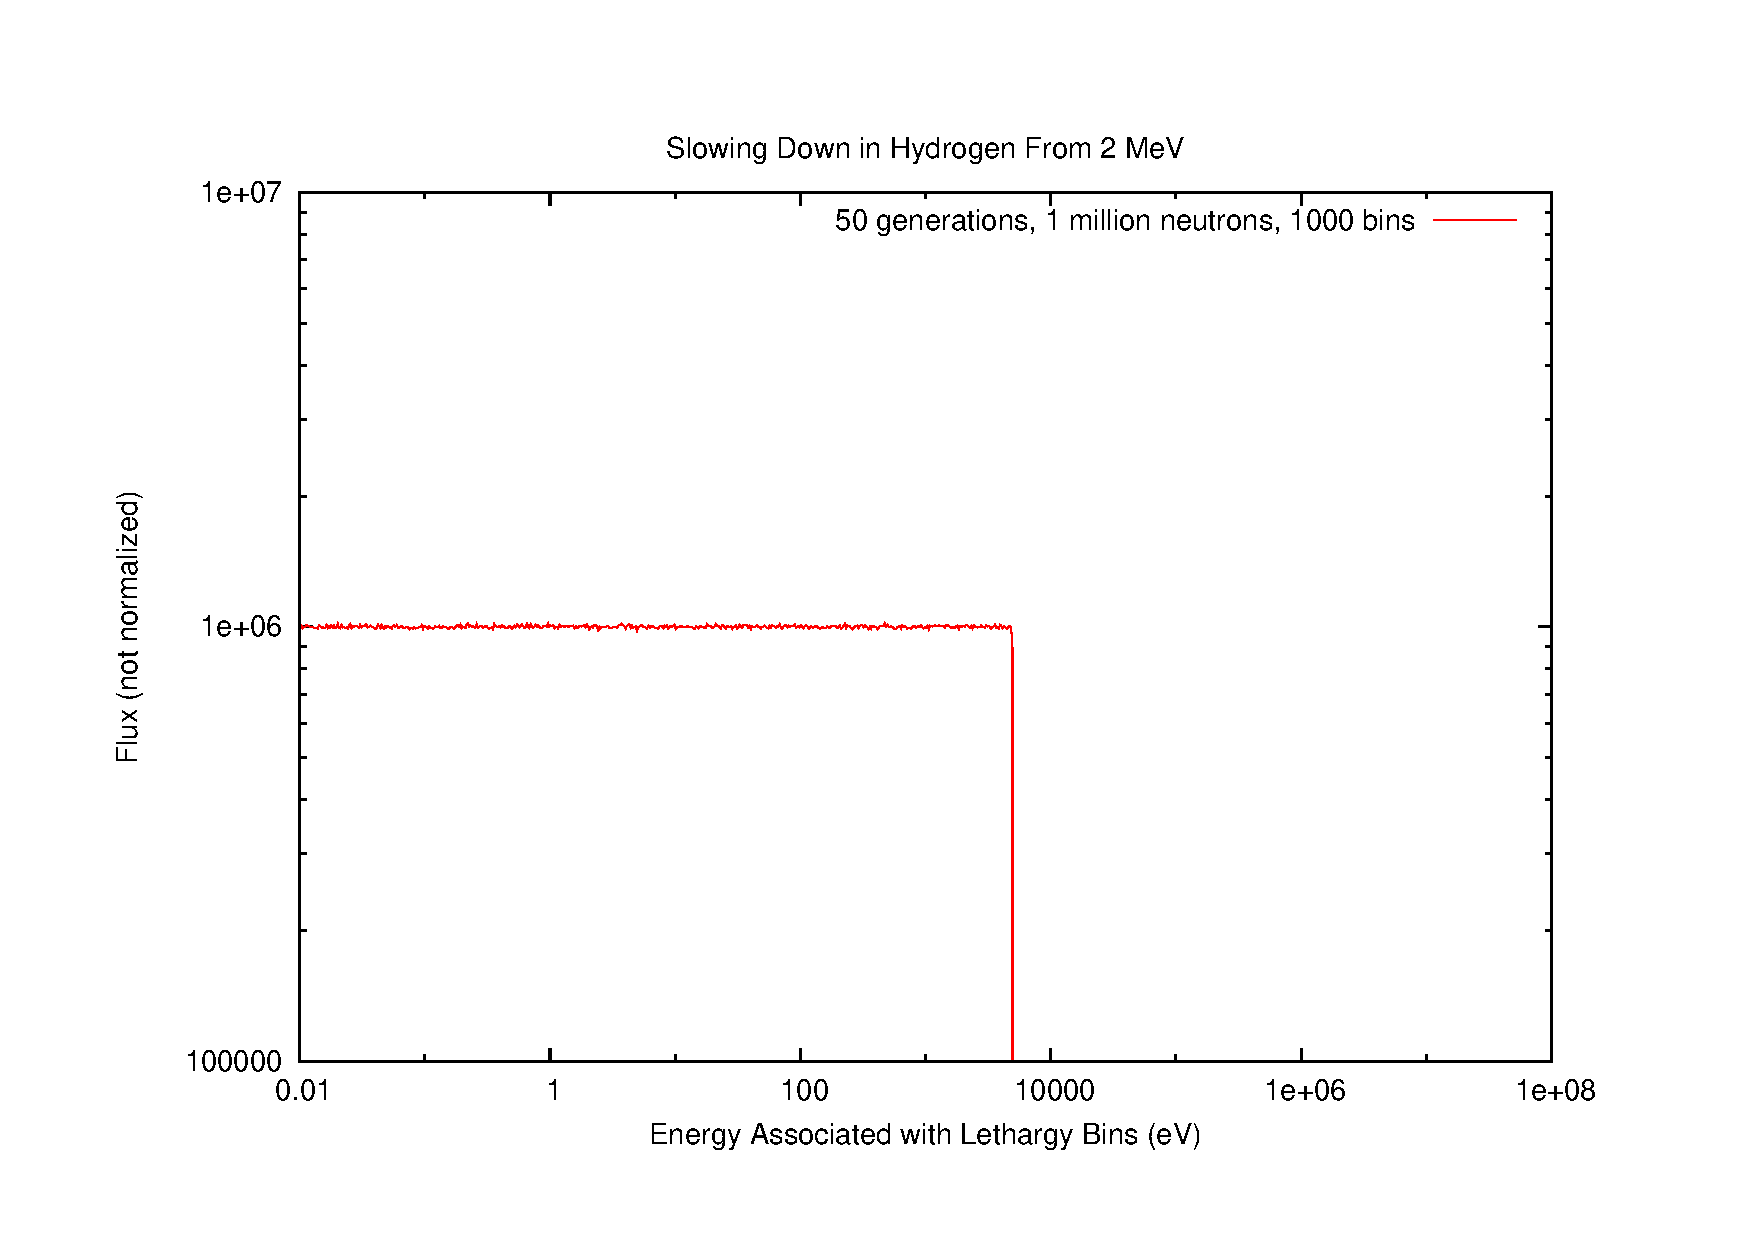
\includegraphics[width=0.3\textwidth]{images/sl-d/spec-1.uncrop.pdf} & asymptotic elastic scattering in hydrogen with source neutrons from 2 MeV \\ 
    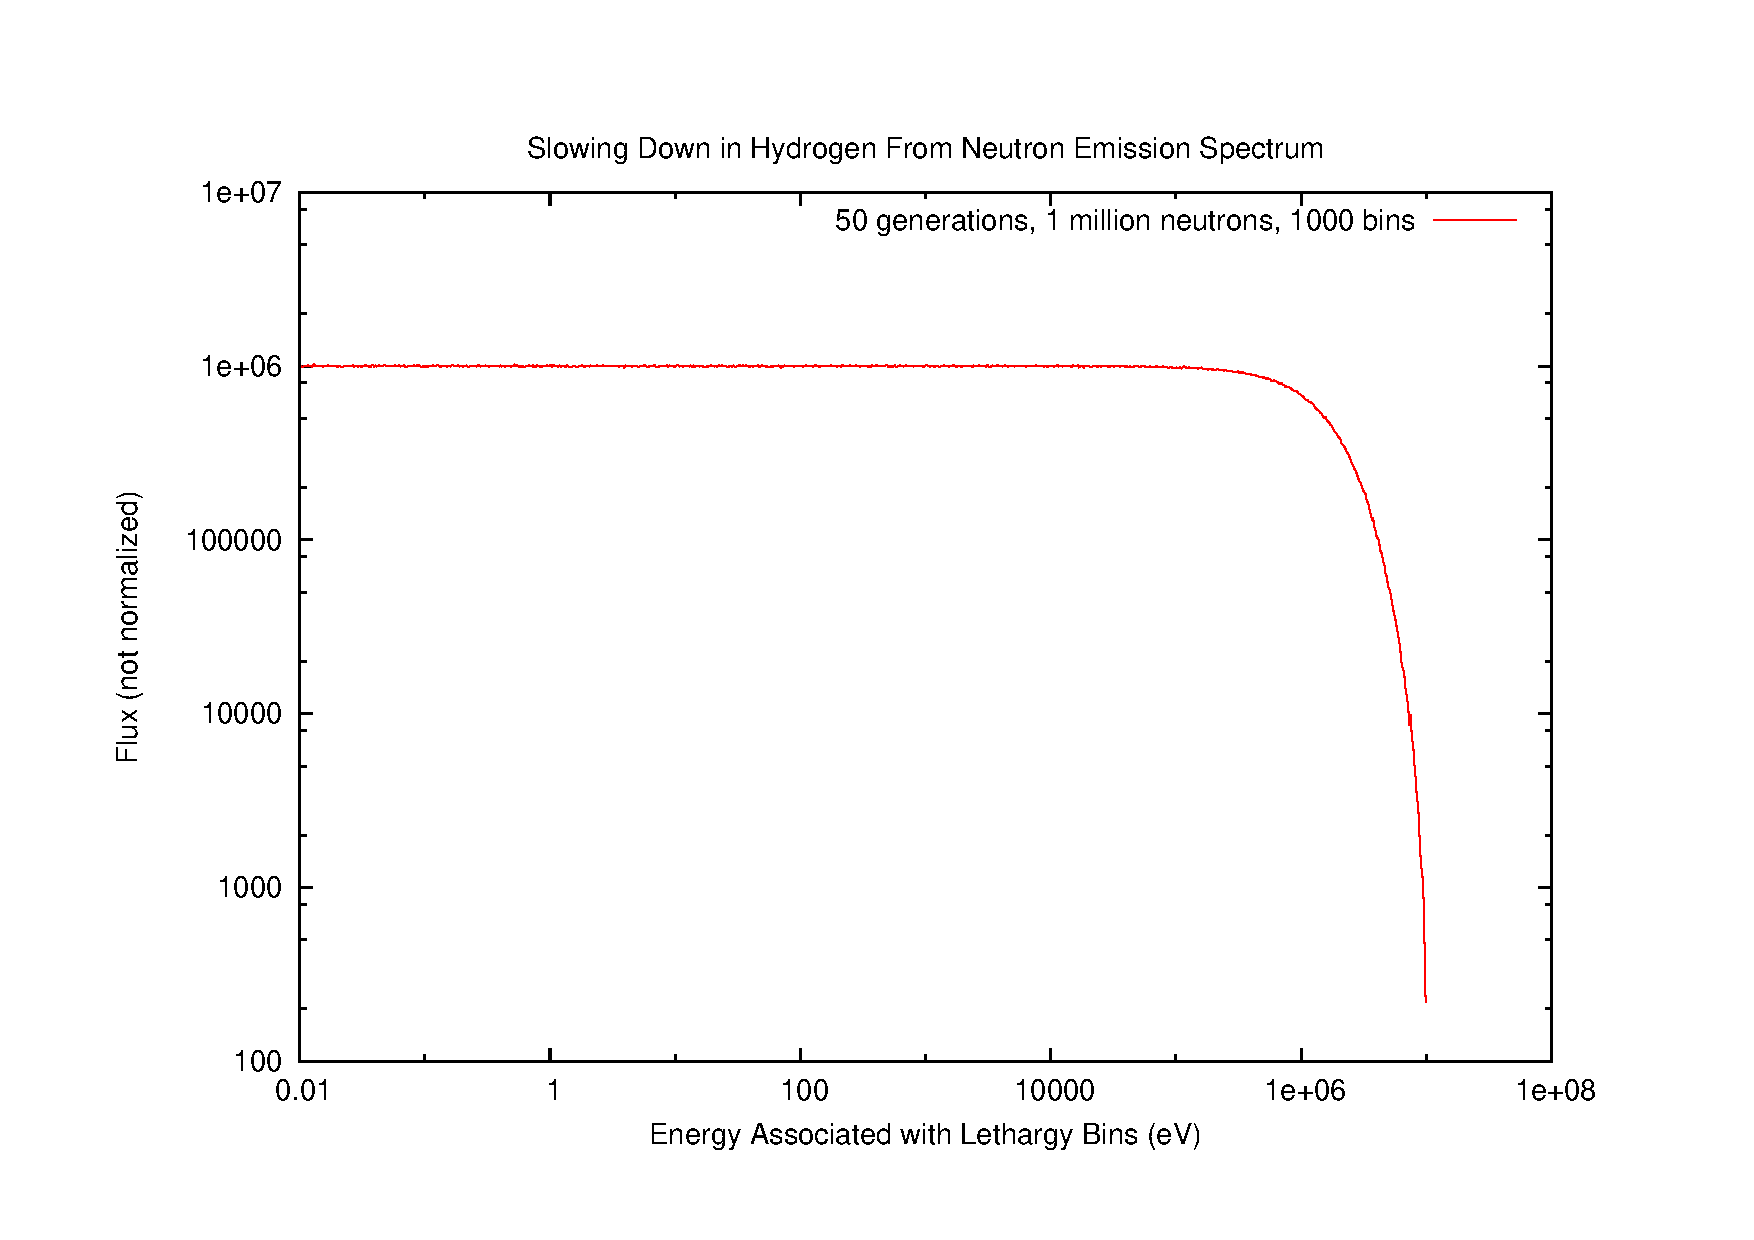
\includegraphics[width=0.3\textwidth]{images/sl-d/spec-2.uncrop.pdf} & replace source neutrons with neutron emission spectrum \\
    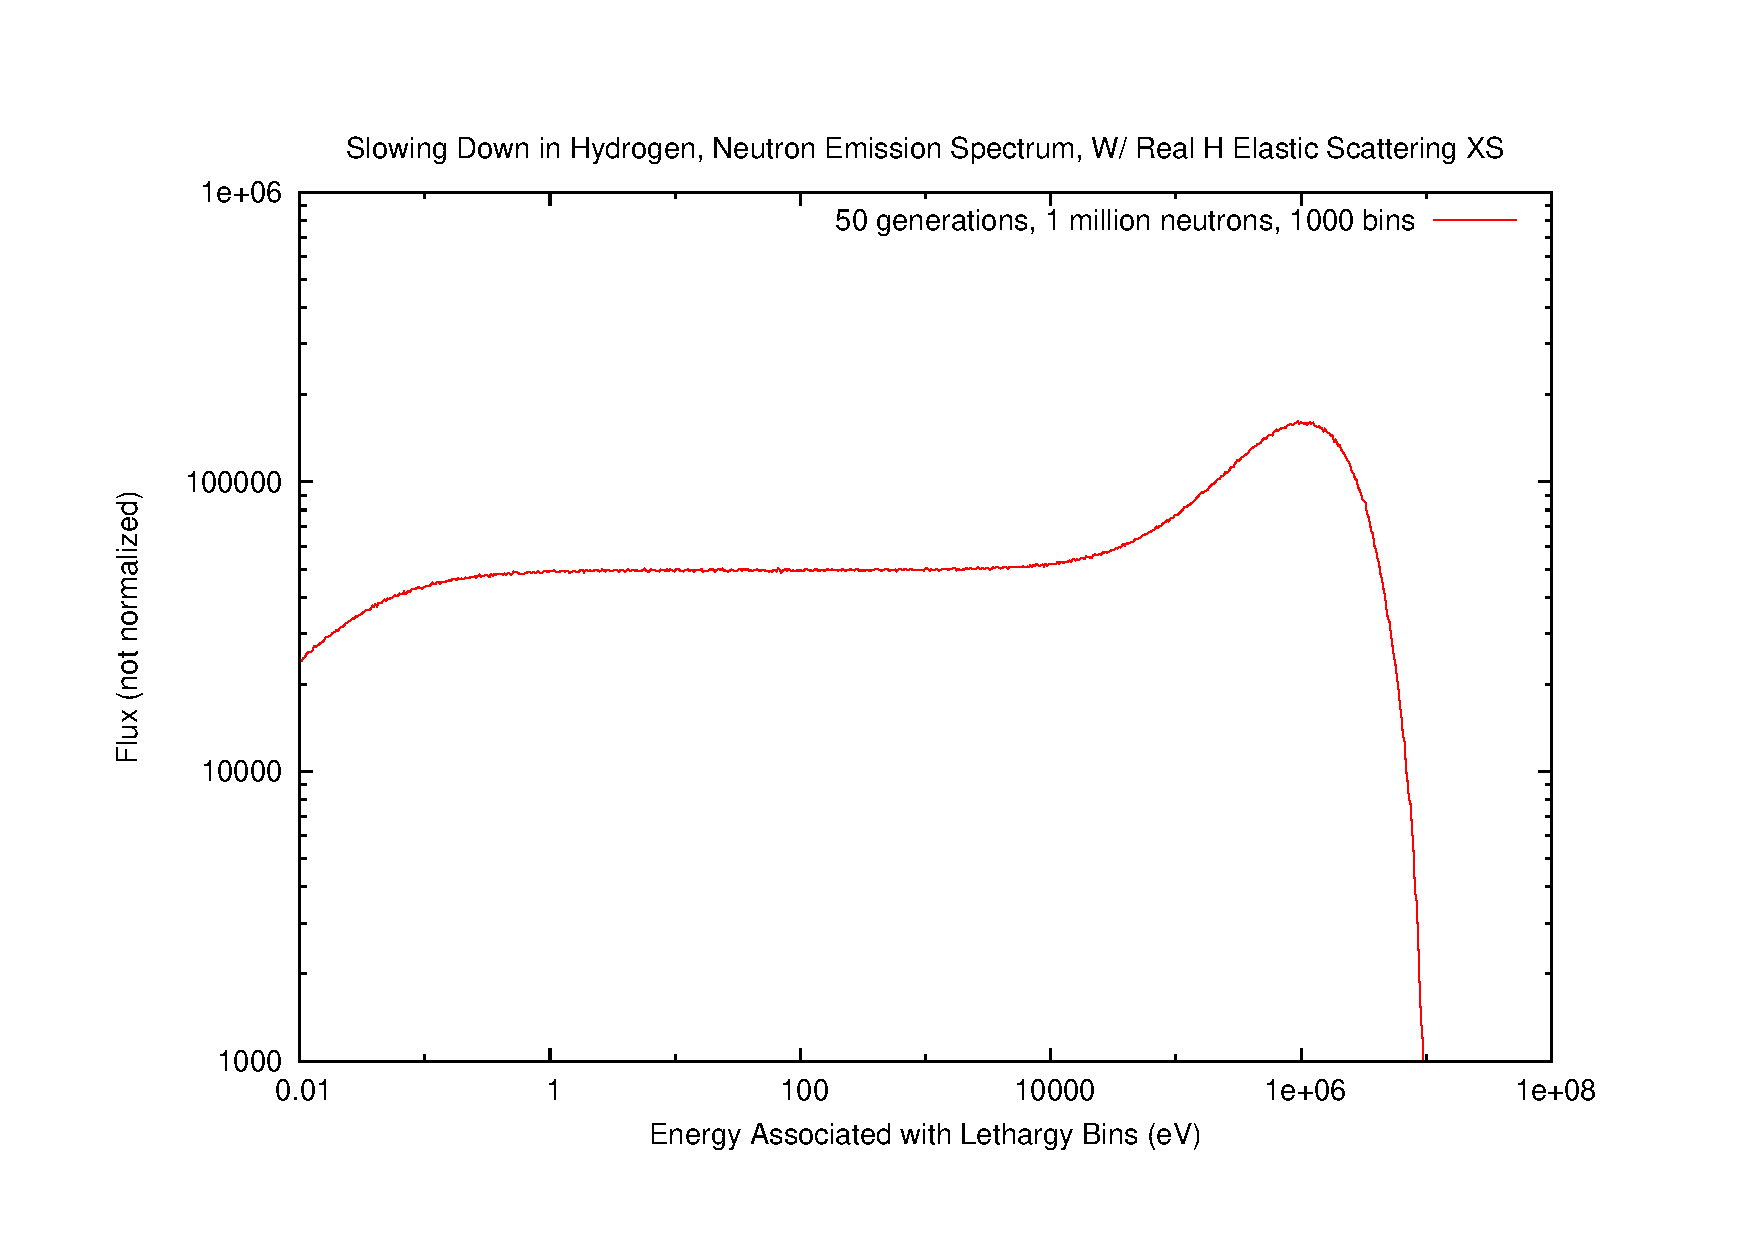
\includegraphics[width=0.3\textwidth]{images/sl-d/spec-3.uncrop.pdf} & add in real H elastic scattering xs (to divide the flux counter by) \\
    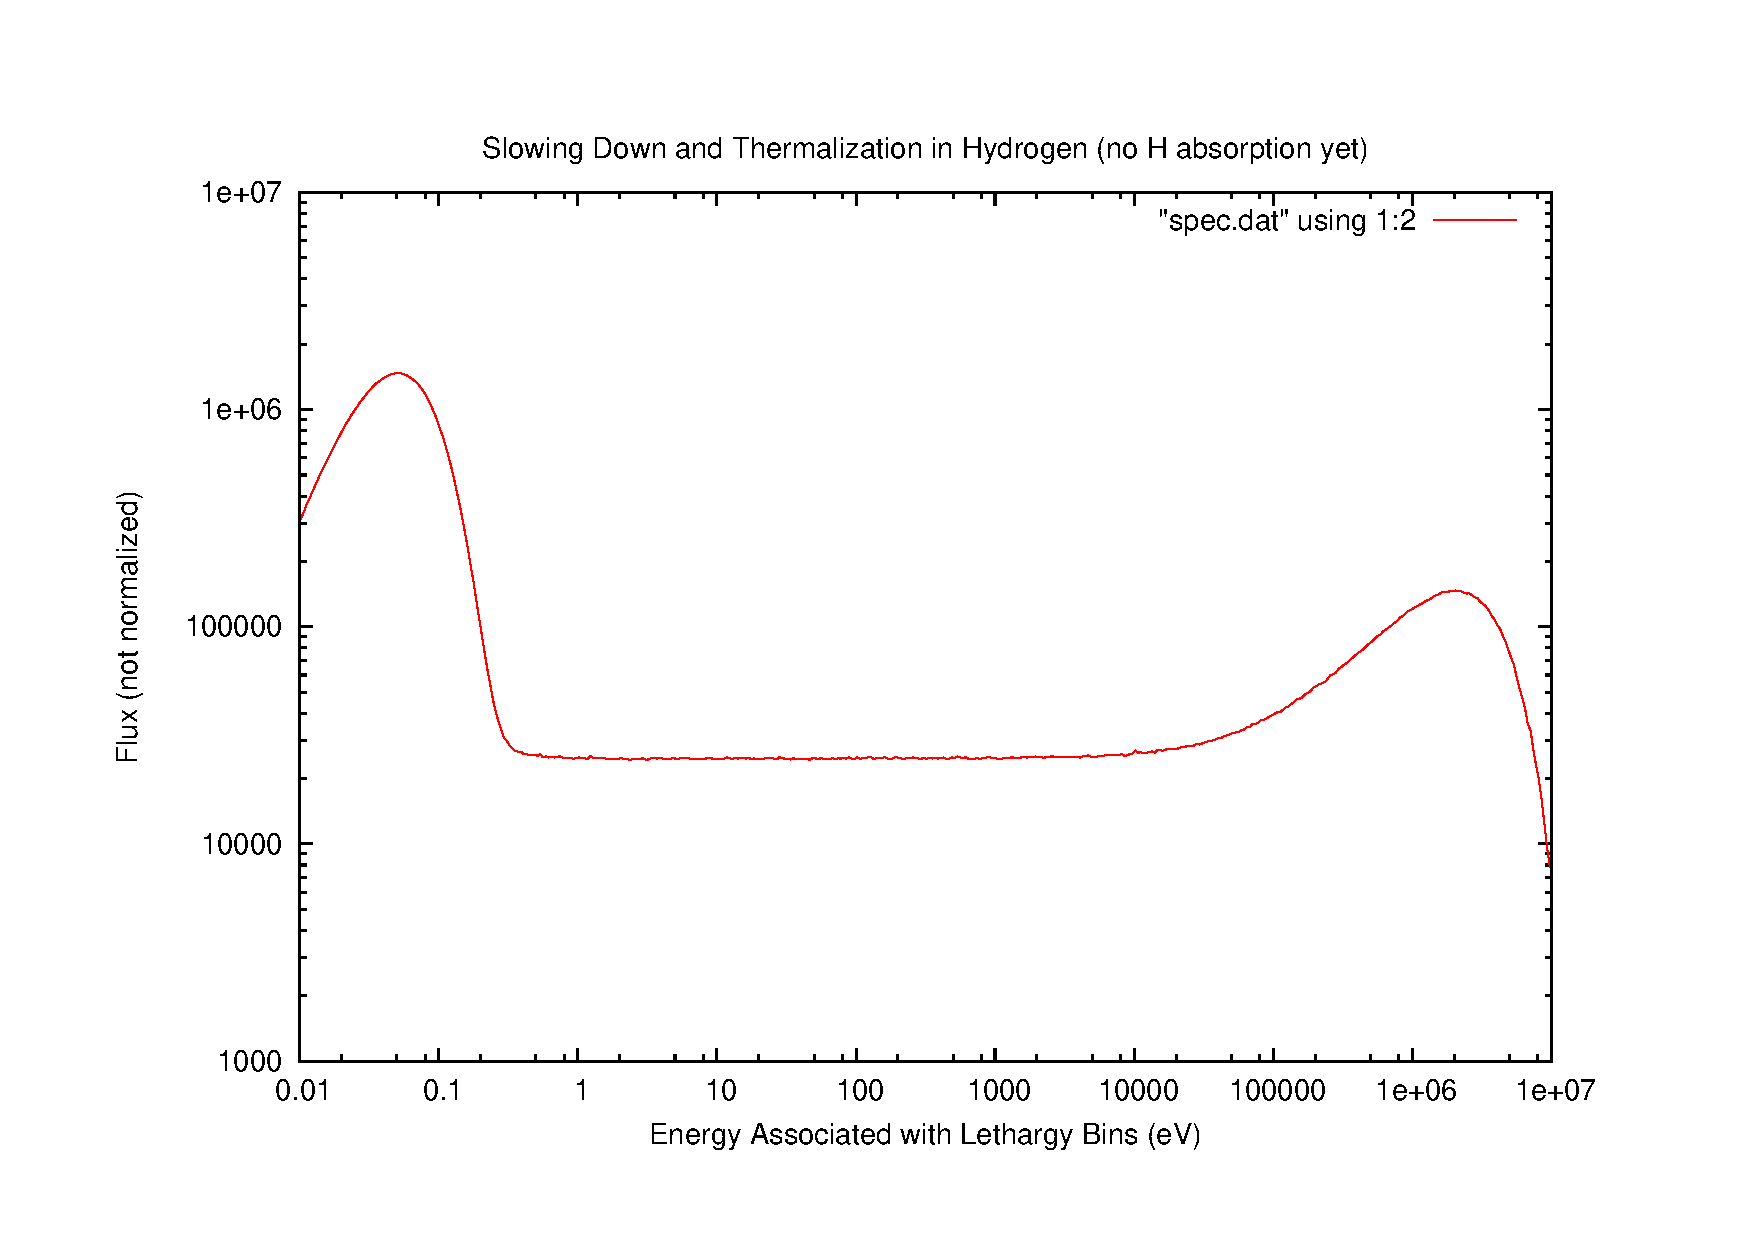
\includegraphics[width=0.3\textwidth]{images/sl-d/spec-4.uncrop.pdf} & add in thermalization in hydrogen ($<$ 4 eV, thermal scattering) \\
    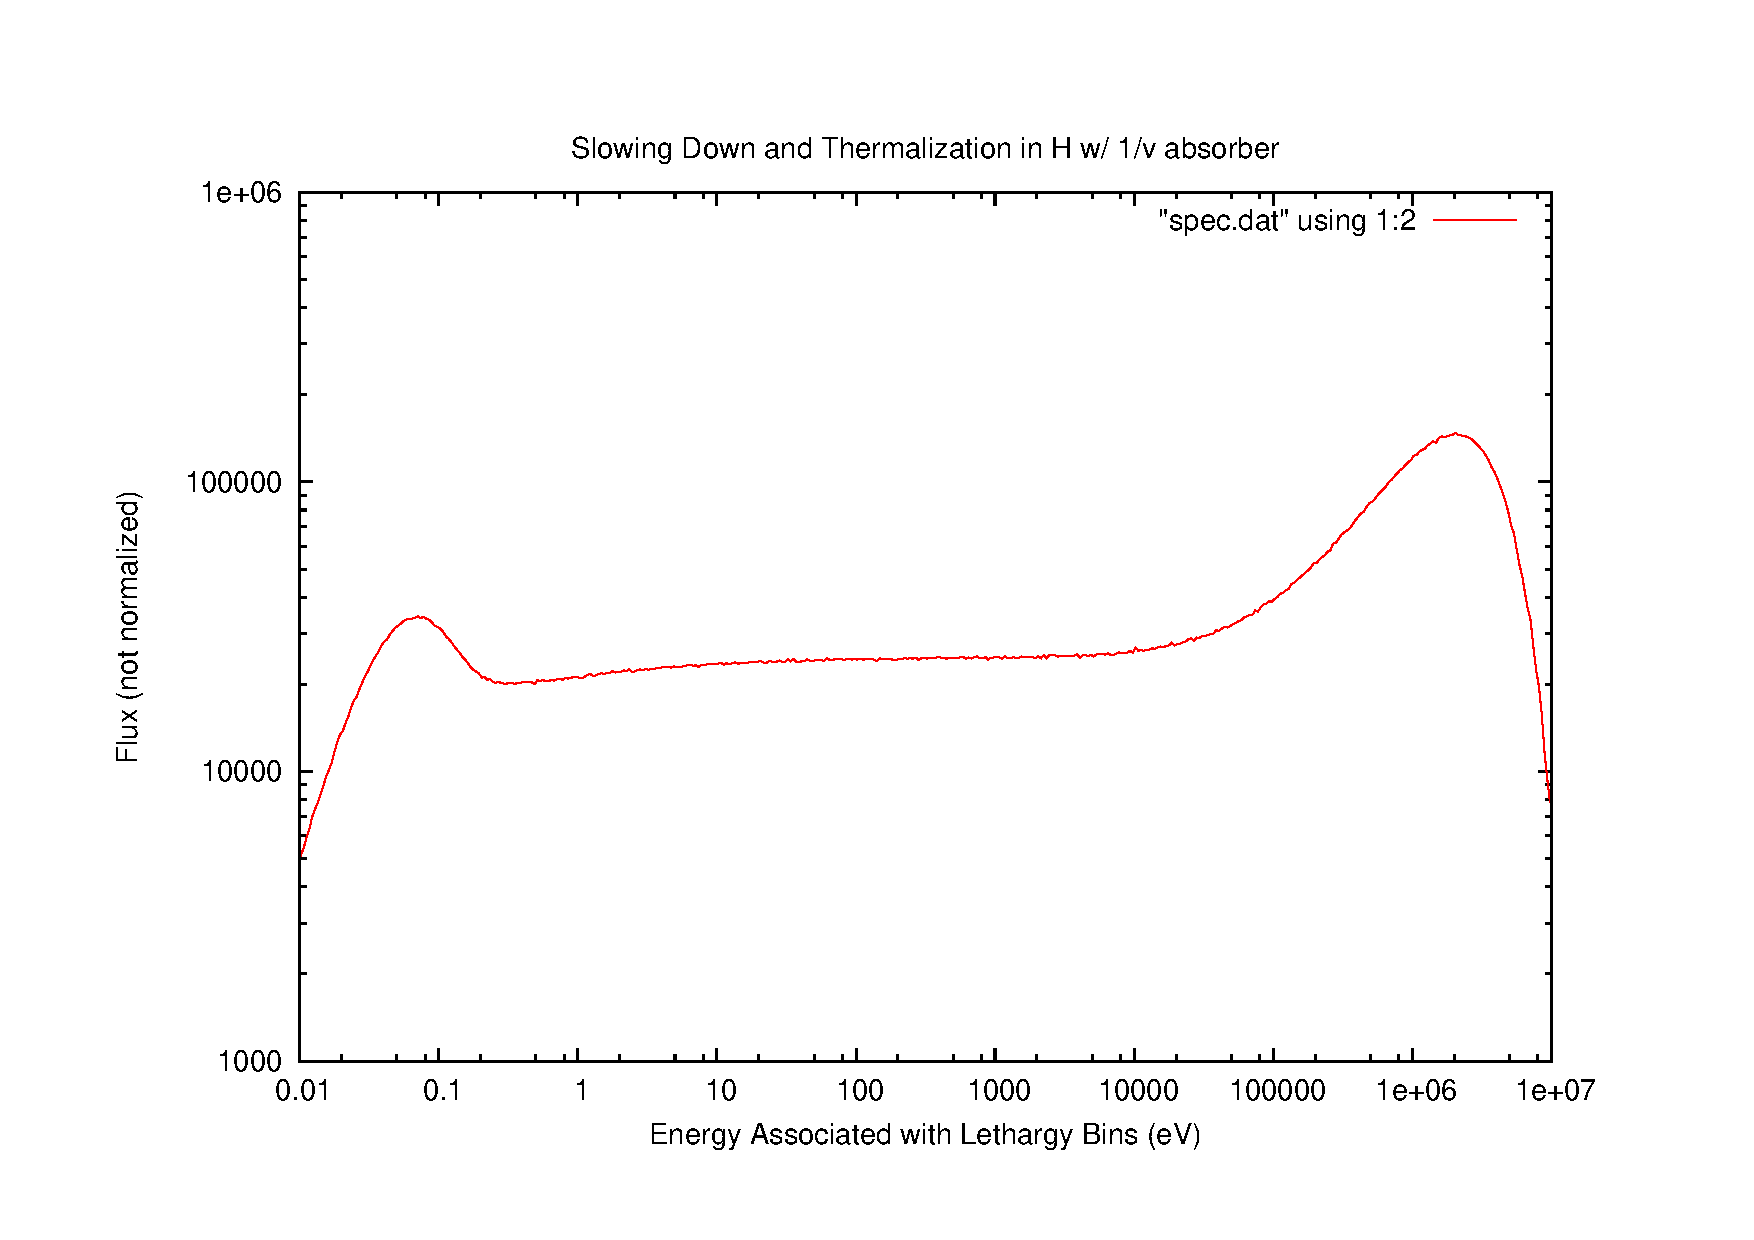
\includegraphics[width=0.3\textwidth]{images/sl-d/spec-5.uncrop.pdf} & add in 1/v H absorber (effective only in the thermal range) \\
    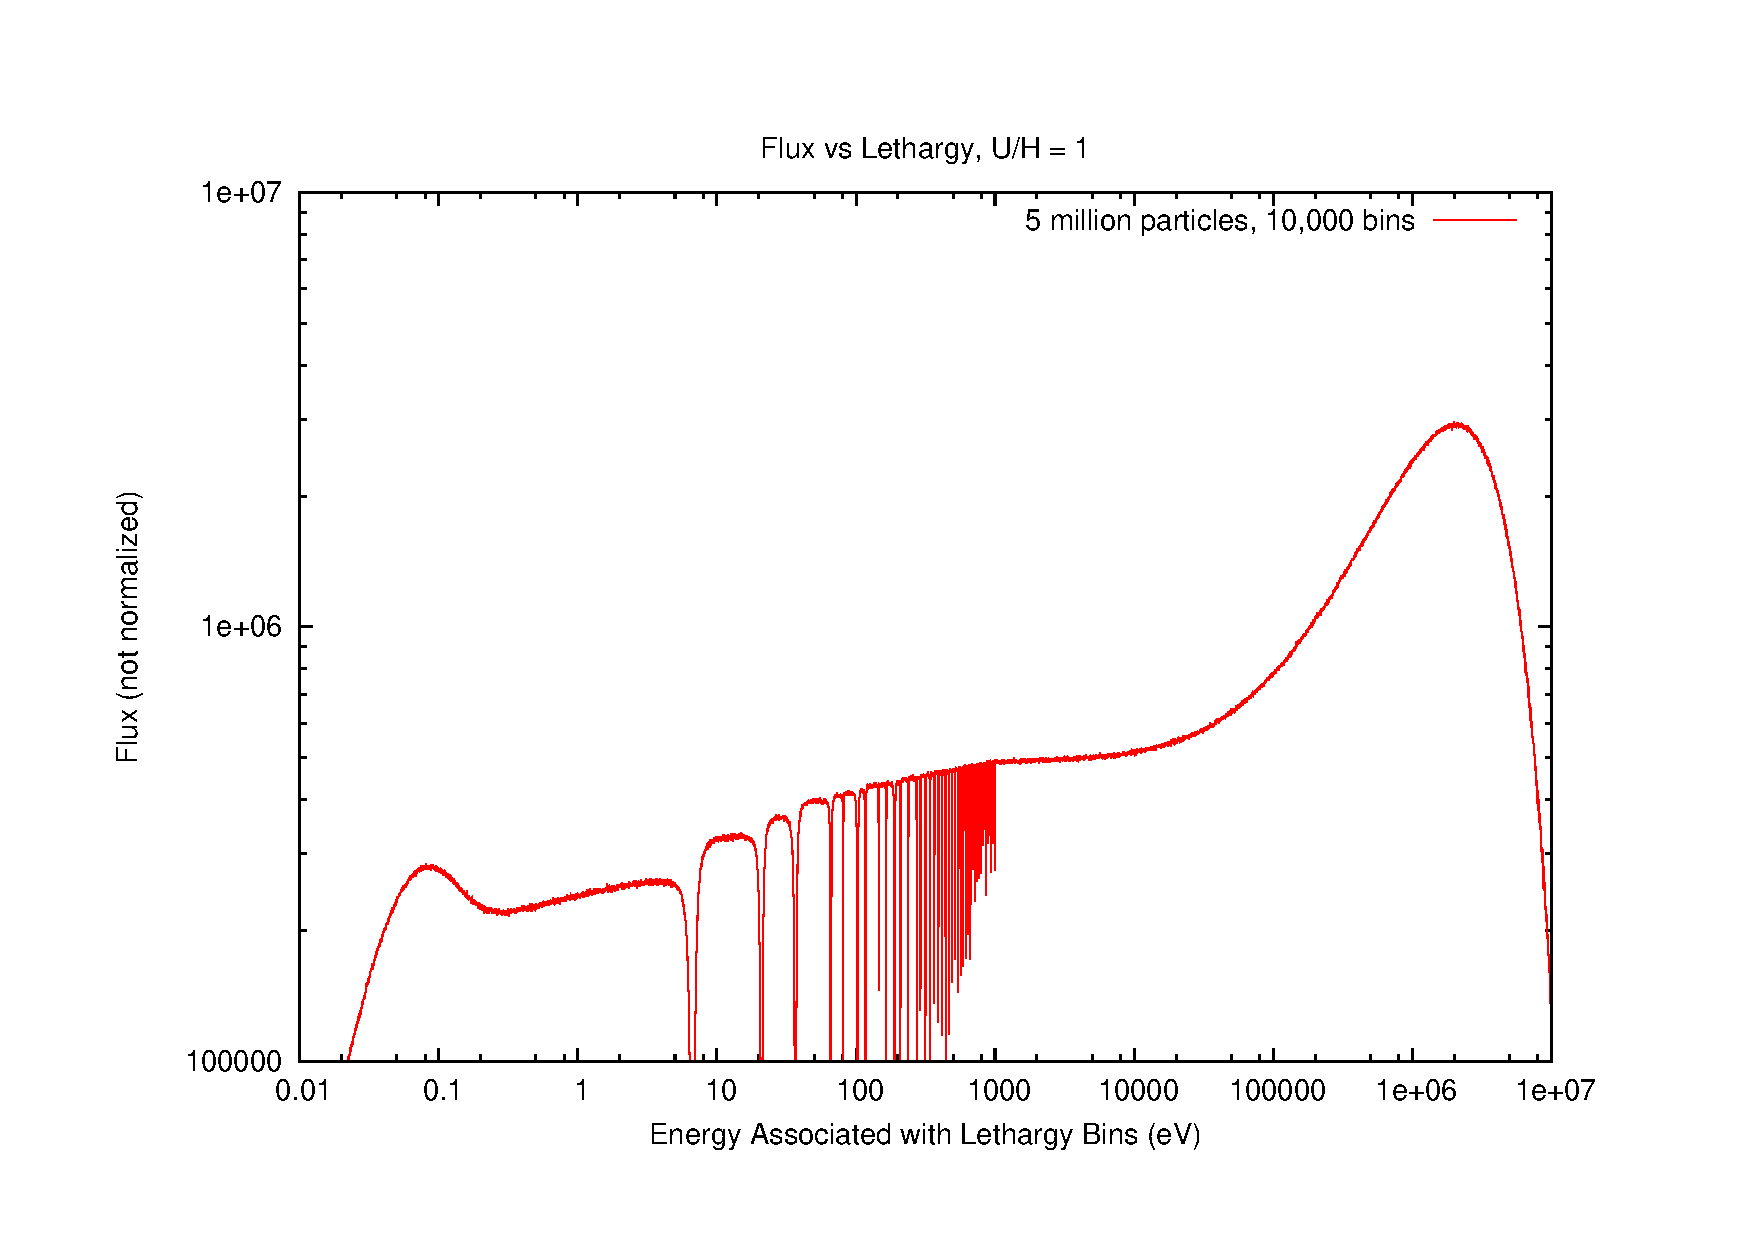
\includegraphics[width=0.3\textwidth]{images/sl-d/spec-7.uncrop.pdf} & add in U238 resonance absorption cross section \\
  \end{tabular}
  \caption{Physics and Their Corresponding Spectra in MC code} \label{plot-MC}
\end{table}

\topic{Concepts I got wrong in Exam 1}
\begin{enumerate}
\item 1/v cross section shape due to thermal motion. [2]
\item Thermal scattering kernel: notice for symmetry; know how to go from pdf to cdf etc. [1]
\item Resonance Integral: only include the resonance cross section, not the potential cross section. [2]
\item Infinite dilute implies that here is no neutrons being absorbed by the resonances. Recall that in HW2 when our U/H is small, the flux is not perturbed by U238 resonances at all, suggesting that the resonance escape probability is one. [1]
\item Calculate effective RI through $\RIeff = \int \sigma_r \phi \frac{1}{E} \dE.$ There is no integration of flux on the bottom (only introduced group xs's definition for the simulation's purpose). [2]
\item Calculate probabilities in 2 region setup. [3]
\item Monte Carlo tallies: U238 absorption rate can be estimated as $\Sum \frac{\Sigma_a}{\Sigma_t}$, the U238 absorption rate per atom is $\Sum \frac{\sigma_a}{\Sigma_t}$. [2]
\end{enumerate}




%%%%%%%%%%%%%%%%%%%%%%%%%%%% Exam 1 Review End %%%%%%%%%%%%%%%%%%%%%%%%%%%%%%%%%%%%%%%%%%





\clearpage
%%%%%%%%%%%%%%%%%%%%%%%%% Qualify Exam Start %%%%%%%%%%%%%%%%%%%%%%%%%%%%
\lecture{Facts For Qualify Exam}
\topic{Basics}
\begin{enumerate}
\item Common units, see Table~\ref{units}.
\begin{table}
  \centering
  \begin{tabular}{|c|c|c|c|} \hline
   $\sigma$ & $\Sigma$ & $\phi = nv$ & $R = \phi \Sigma$  \\ \hline
   $\cm^2$ & $1/\cm$ & $\frac{n}{\cm^2 \s}$ & $\frac{\mathrm{reactions}}{\cm^3 \s}$ \\ \hline
  \end{tabular}
  \caption{Units of Common Terms} \label{units}
\end{table}
\item Fast flux in hydrogen is around $10^{14}$ n/cm$^2$s, and on the order of $10^{12}$n/cm$^2$s for thermal flux. 
\item Average fission neutron energy: 2 MeV; average peak fission energy: 1 MeV; see fission sepctrum. 
\item Core decay heat after 1 day is about 1\% rated. 
\item Constants to know: 1u = 931.5 MeV. 
\item The effect of U238 energy self-shielding is about an effect of 10, that is, going from infinite dilution to U/I = 0.1. 
\end{enumerate}

\topic{Cross Section}
\begin{enumerate}
\item* If the neutron cross section is independent of energy at 0K, at 1200K the cross section would have a 1/v energy shape because of thermal motion. 
  
\item* Resonance absorption cross section dominates resonance scattering cross section most of the time (except U238). 

\item* Fission cross section: U235 fission xs at 0.1 eV and 300K is about 200 barns (200-300 barns); Pu239 fission xs is about 475 barns (380-570 barns). Hence in thermal reactors, Pu absorption should be about twice that of uranium. 

\item Elastic scattering cross section as in Figure~\ref{scatter-xs}
\begin{figure}
  \centering
  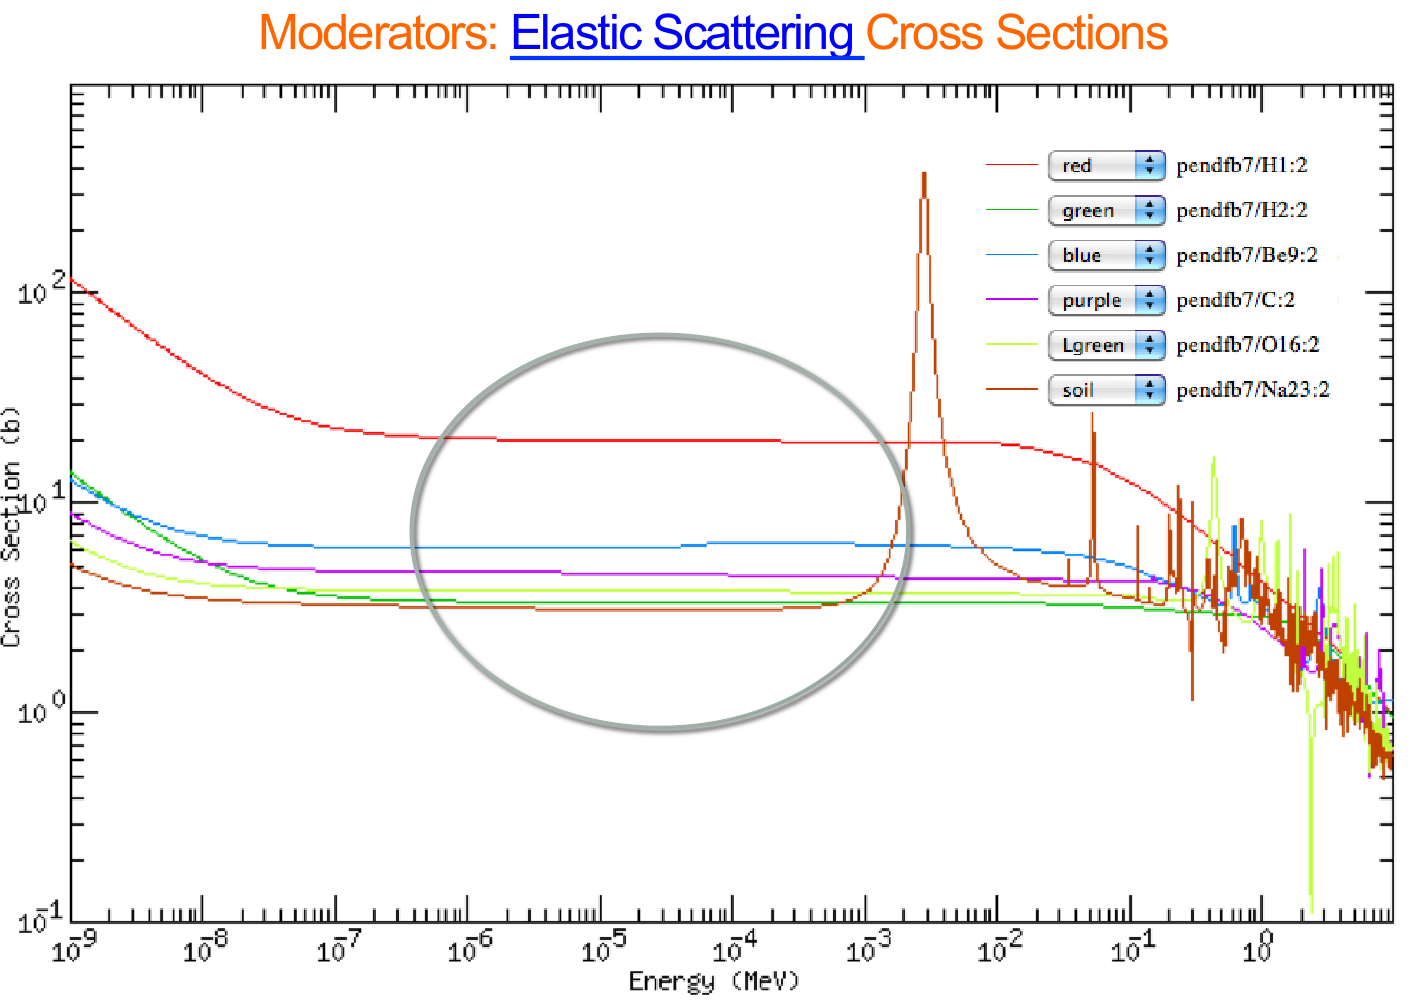
\includegraphics[width=6in]{images/intro/scatter-xs-moderator.png}
  \\
  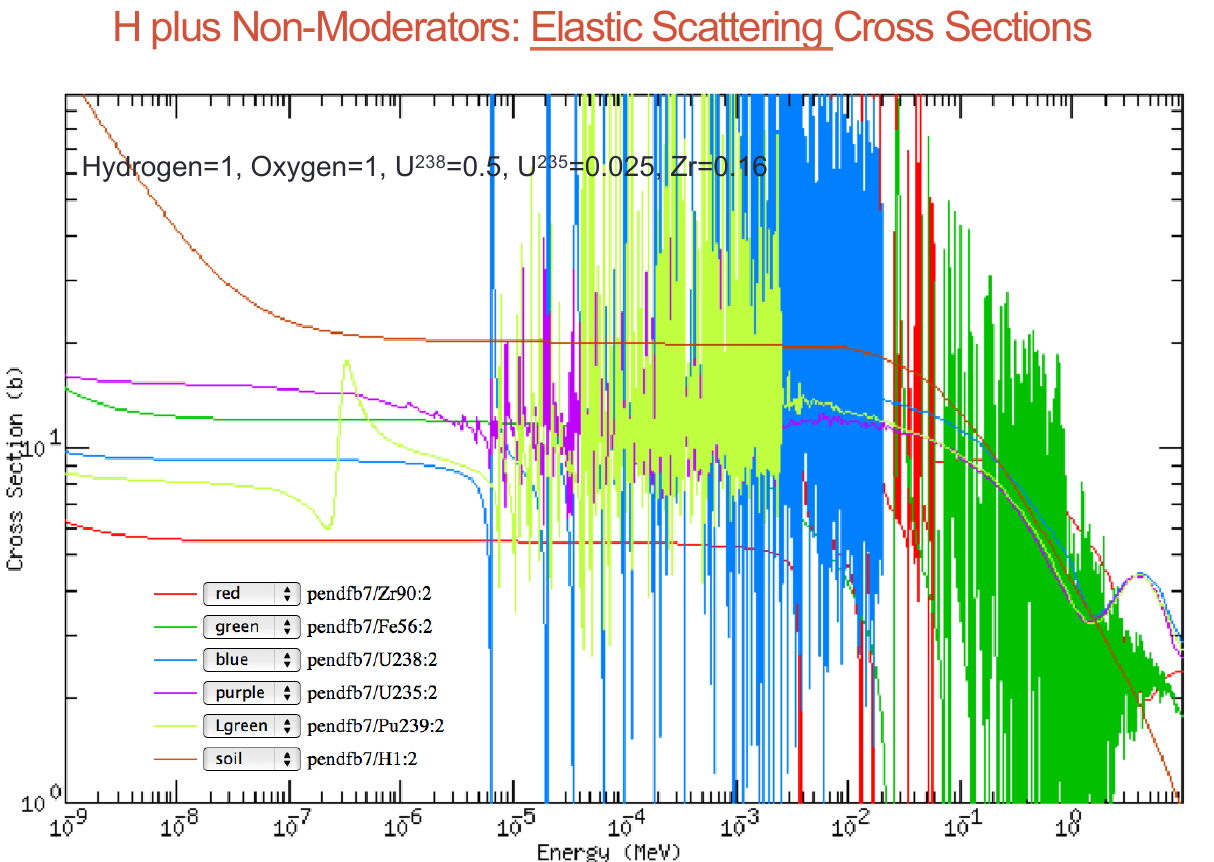
\includegraphics[width=6in]{images/intro/scatter-xs-LWR.png}
  \caption{Elastic Scattering Cross Sections} \label{scatter-xs}
\end{figure}

\item Capture cross section as in Figure~\ref{capture-xs}: 
  \begin{figure}
    \centering
    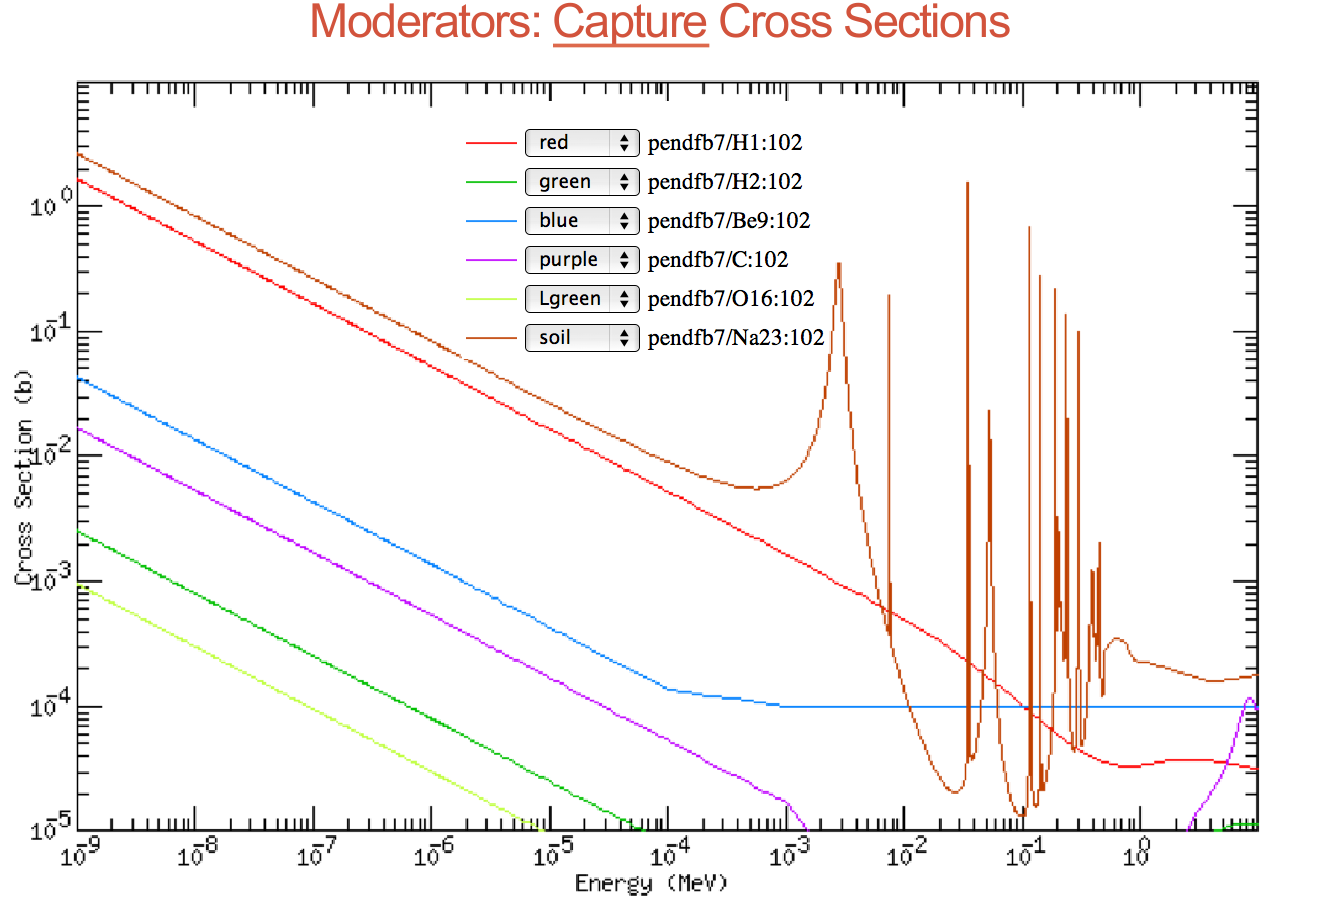
\includegraphics[width=6in]{images/intro/capture-xs.png}
    \\
    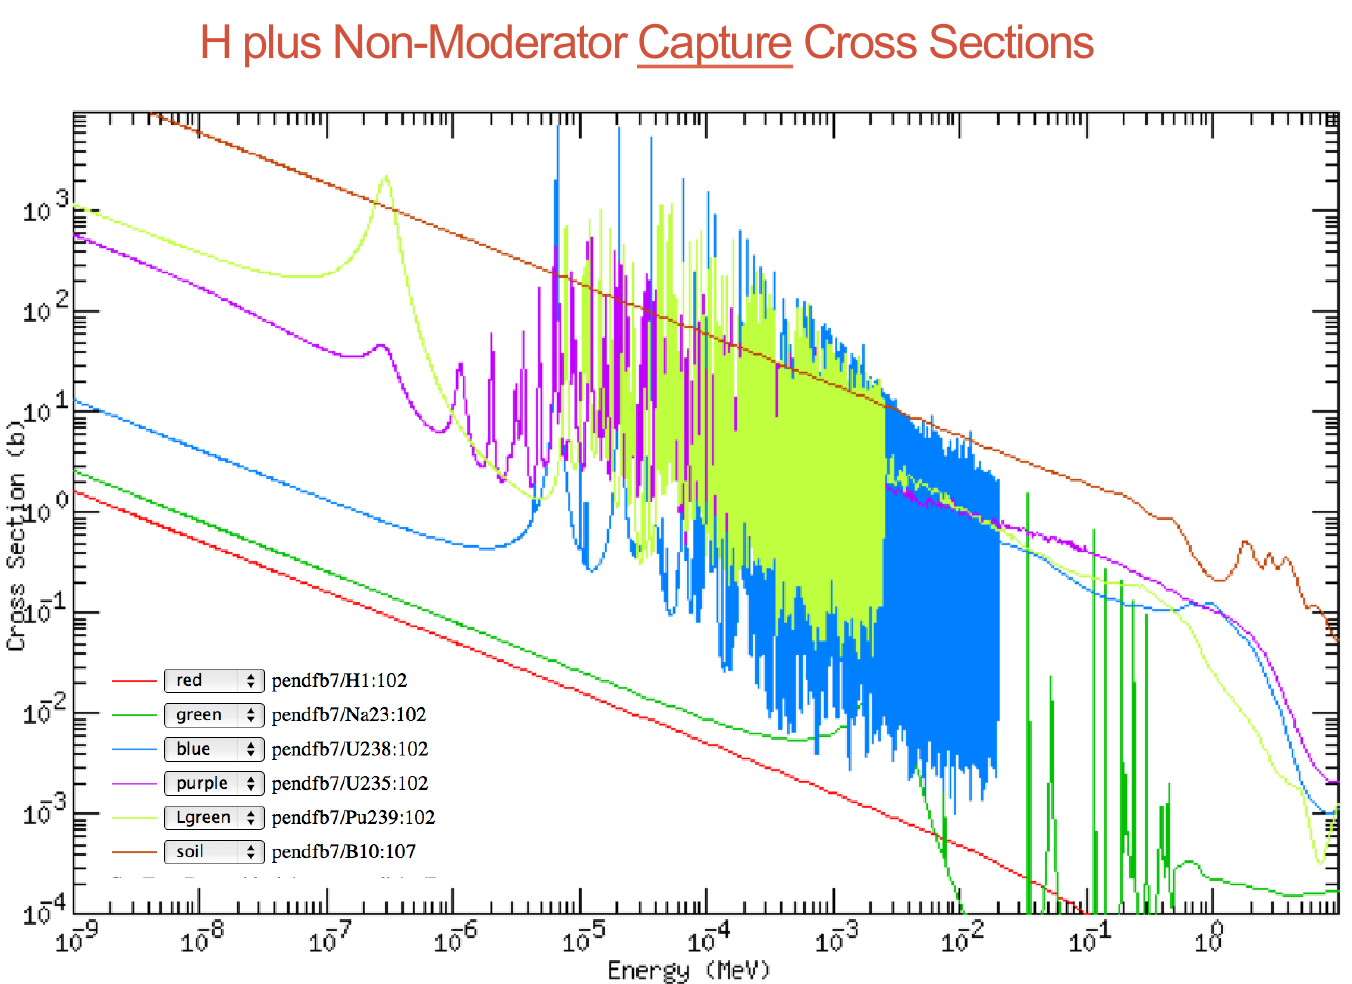
\includegraphics[width=6in]{images/intro/capture-xs-2.png}
    \caption{Capture Cross Section} \label{capture-xs}
  \end{figure}
  \begin{enumerate}
  \item H has no resonance; it has the highest scattering xs in LWR, so we can ignore any other isotopic's neutron scattering.   
  \item Na has a huge resonance in 23 keV, and more resonances at higher energies because it is a heavy isotope.
  \item Near zero energy,
    \eqn{ \sigma(E\to 0) \propto \sqrt{\frac{kT}{AE}}    }
  \item Resonance at 6 to 7 eV: U238. 
  \item U235's thermal elastic xs is larger than 238's, and they both have resonance around the same range.   
  \item A small resonance at .3 eV: Pu239 (its signiture is a super low energy scattering xs). 
  \end{enumerate}

\item Given an unknown material type, all we care is to count the nucleus density of each material and look at it's xs. 
\end{enumerate}

\topic{Kinetics}
\begin{enumerate}
\item One group k-infinity: in one group $k_{\infty}$ only depends on cross sections $k_{\infty} = \frac{\nu \Sigma_f}{\Sigma_a}$ and has no flux dependency. The flux is buried in the calculation of cross section.
\item Two group k-infinity: we start with neutron balance equation:
\begin{align}
\frac{\nu \Sigma_{f1}}{k_{\infty}} \Phi_1 - \Sigma_{a1} \Phi_1 - \Sigma_{s12} \Phi_1 + \frac{\nu \Sigma_{f2}}{k_{\infty}} \Phi_2 + \Sigma_{s21} \Phi_2 &= 0 \\
\Sigma_{s12} \Phi_1 - \Sigma_{s21} \Phi_2 - \Sigma_{a2} \Phi_2 &= 0 
\end{align}
Typically what we do is to write it in a matrix form and solve for a coupled system. But even better, we can define the \hi{effective removal rate} $\bar{\Sigma}_{s12}$, and re-write the two-group balance equation: 
\begin{align}
\frac{\nu \Sigma_{f1}}{k_{\infty}} \Phi_1 - \Sigma_{a1} \Phi_1 - \bar{\Sigma}_{s12} \Phi_1 + \frac{\nu \Sigma_{f2}}{k_{\infty}} \Phi_2 &= 0 \\
\bar{\Sigma}_{s12} \Phi_1- \Sigma_{a2} \Phi_2 &= 0 
\end{align}
Then we can solve for $\frac{\Phi_1}{\Phi_2}$ from the second equation in terms of cross section, plug in the first equation, and get $k_{\infty}$ from there. Notice that we only know the relative magnitude of $\Phi$ and $\Phi_2$. 


\end{enumerate}
%%%%%%%%%%%%%%%%%%%%%%%%% Qualify Exam End %%%%%%%%%%%%%%%%%%%%%%%%%%%%


\end{document}
